\section{10/15/2019}

\subsection{Finishing up linear regression}

We first collect some useful facts about linear regression.
First, by optimality of $\theta^*(p)$
\begin{align}
  0
  &= \frac{1}{2} \left.\frac{\partial L(p, \theta)}{\partial \theta} \right\rvert_{\theta = \theta^*(p)}
  = \ex[X (Y - \braket{\theta^*(p), X}) ]
  = \ex[ X Z ]
\end{align}
Furthermore, if the regression has an intercept term (e.g.\ if one coordinate
$X_i$ were deterministically a constant) then $\ex[Z] = 0$.

\textbf{Caution}: We can have $\ex[Z \mid X] \neq 0$, which is the situation
when residuals are correlated with $X$. For example, consider the following
scenario:

\begin{figure}[H]
  \begin{center}
    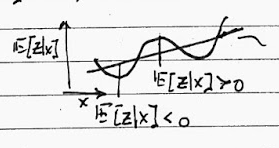
\includegraphics[width=0.4\textwidth]{figures/10-15-1.png}
  \end{center}
\end{figure}

The fact that $\ex[X Z] = 0$ is what gives us the quadratic form representation
for excess loss:
\begin{align}
  L(q, \theta)
  &= \ex_q[(Y - \braket{\theta, X})^2] - \ex_q[(Y - \braket{\theta^*(q), X})^2] \\
  &= \ex_q\left[
    \braket{\theta, X}^2
    + \braket{\theta^*(q), X}^2
    - 2 Y \braket{\theta - \theta^*(q), X}
  \right] \\
  &= \ex_q\left[
    \braket{\theta - \theta^*(q), X}^2
    - 2 \braket{\theta^*(q), X} \braket{X, \theta^*(q) - \theta}
    + 2 Y \braket{X, \theta^*(q) - \theta}
  \right] \\
  &= \ex_q\left[
    \braket{\theta - \theta^*(q), X}^2
    + 2 (Y - \braket{\theta^*(q), X}) \braket{X, \theta^*(q) - \theta}\
  \right] \\
  &= \ex_q\left[
    \braket{\theta - \theta^*(q), X}^2
    + 2 \cancelto{0}{Z \braket{X, \theta^*(q) - \theta}}
  \right] \\
  &= \|\theta - \theta^*(q)\|_{S_q}^2
\end{align}
In this setting, the resilience conditions we need to show are
\begin{itemize}
  \item $\cG_\downarrow$: $\|\theta^*(p) - \theta^*(r)\|_{S_r}^2 \leq \rho$
  \item $\cG_\uparrow$: $\|\theta^*(r) - \theta)\|_{S_r}^2 \leq \rho \implies \|\theta^*(p) - \theta\|_{S_p}^2 \leq 5 \rho$
\end{itemize}
Last time we showed that $\cG_\uparrow$ is implied by
$\cG_\downarrow$ and we took for granted $\|S_r^{-1/2} \ex_r[X Z]\|_2 = \|\ex_r[X Z]\|_{S_r} \leq 2
\sigma \sqrt{\eps}$. This was required for verifying $\cG_\downarrow$ because
by \cref{eq:linreg-second-moment-diff-theta-star}
and \cref{lem:linreg-second-moment-close}
\begin{align}
  \|\theta^*(p) - \theta^*(r)\|_{S_r}^2
  &= \| \ex_r[X Z]\|_{S_r}^2
  \leq 2 \| \ex_r[X Z]\|_{S_p}^2
  = 2 \| S_p^{-1/2} \ex_r[X Z]\|_2^2
\end{align}
The RHS is now just ordinary mean resilience in the $\ell_2$ norm
(note that when $r = p$ the mean is zero), so we can
control it by controlling the covariance and applying
\cref{eg:bdd-cov-resilient}.
By bounding covariance with second moment and using the bounded
noise hypothesis:
\begin{align}
  \Cov_p[S_p^{-1/2} X Z]
  &\leq \ex_p[S_p^{-1/2} X Z^2 X^\top S_p^{-1/2}]
  = S_p^{-1/2} \ex[X Z^2 X^\top] S_p^{-1/2} \\
  &\leq \sigma^2 S_p^{-1/2} \ex[X X^\top] S_p^{-1/2}
  = \sigma^2 I
\end{align}

\subsection{Linear Classification}

Let $(X,Y) \in \RR^d \times \{\pm 1\}$. We can consider the
\emph{classification loss}
\begin{align}
  L(p, \theta) = \Pr_p[Y \neq \sgn\braket{\theta, X}]
\end{align}
or \emph{hinge loss}
\begin{align}
  B(p, \theta) = \ex_{X, y} \max(1 - \braket{\theta, x}y, 0)
\end{align}

\begin{proposition}
  Suppose $p$ satisfies
  \begin{enumerate}
    \item $\ex_{(X,Y) \sim p} \max (1 - y \braket{\theta^*, x}, 0) \leq (1 - \eps) \rho_1$
    \item For all $\theta$ satisfying
      \begin{align}
        \Pr[y \braket{\theta, X} \leq \frac{1}{2}] \leq \eps + 2(1-\eps) \rho_1
      \end{align}
      we have
      \begin{align}
        \Pr[y \braket{\theta, X} \leq 0] \leq \rho_2
      \end{align}
  \end{enumerate}
  Then $p$ is $(\rho_1, \rho-2, \eps)$ resilient.
\end{proposition}
\todo{which loss}?

\begin{proof}
  HW \todo{add when done}
\end{proof}

\begin{remark}
  The second condition is a statement about the rate of tail decay.
  It says that once the tail starts to decay, then it falls off very fast.

  Figure 10.15.XX

  Compare this to bounded variance, which was stronger and required the probability
  mass to be tightly concentrated (i.e.\ tails both fall off very fast and start
  to fall off close to the mean).
\end{remark}
